\begin{frame}{Titulo}

\begin{figure}[htbp]
\centering
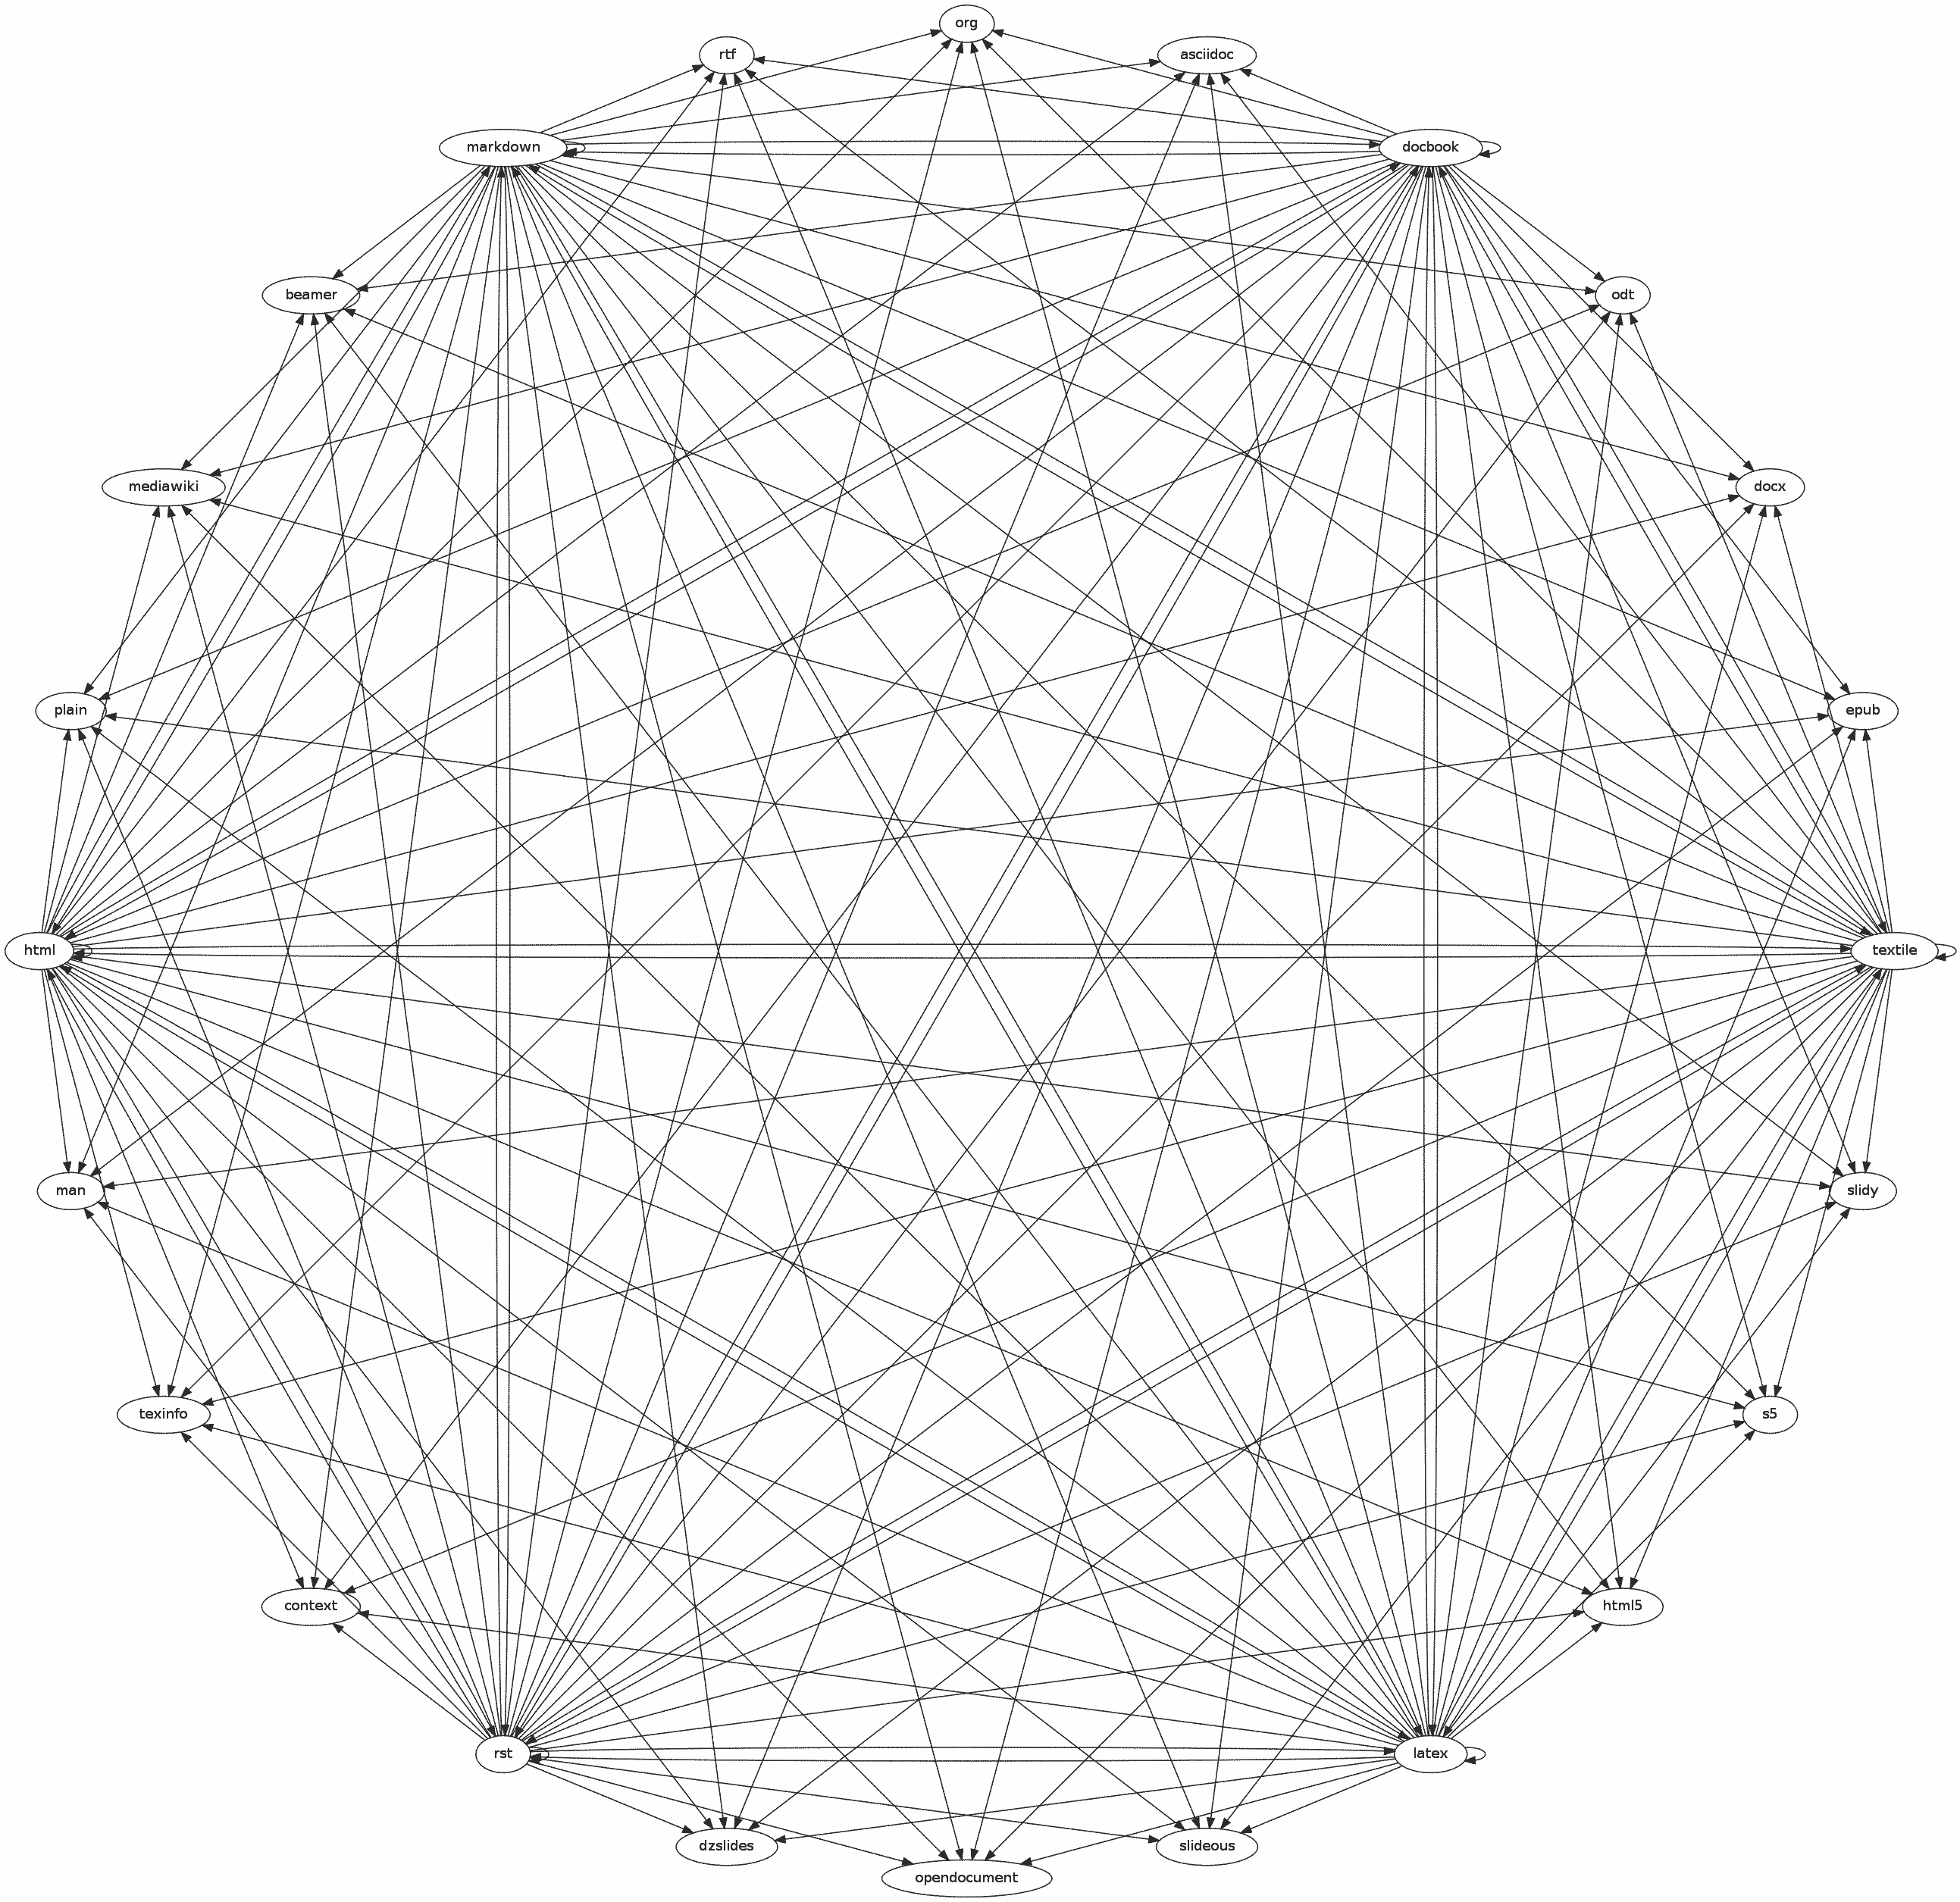
\includegraphics{images/diagram}
\end{figure}

\end{frame}

\begin{frame}{NCBI}

\begin{itemize}
\item
  \textbf{National Center for Biotechnology Information} (NCBI)
  \url{http://www.ncbi.nlm.nih.gov/}
\item
  part of the United States National Library of Medicine (NLM)
  \url{https://www.nlm.nih.gov/}
\item
  a division of the National Institutes of Health (NIH)
  \url{http://www.nih.gov/}
\end{itemize}

\end{frame}

\begin{frame}{Resources}

Databases of biomedical and genomic information for all organisms:

\begin{itemize}
\itemsep1pt\parskip0pt\parsep0pt
\item
  Submission

  \begin{itemize}
  \itemsep1pt\parskip0pt\parsep0pt
  \item
    GenBank
  \end{itemize}
\item
  Databases

  \begin{itemize}
  \itemsep1pt\parskip0pt\parsep0pt
  \item
    GenBank
  \item
    \textbf{RefSeq}
  \item
    \ldots{}
  \end{itemize}
\item
  Downloads

  \begin{itemize}
  \itemsep1pt\parskip0pt\parsep0pt
  \item
    FTP sites
  \item
    PubMed
  \end{itemize}
\item
  Tools

  \begin{itemize}
  \itemsep1pt\parskip0pt\parsep0pt
  \item
    Basic Local Alignment Search Tool (BLAST)
  \item
    \ldots{}
  \end{itemize}
\end{itemize}

See: \url{http://www.ncbi.nlm.nih.gov/guide/all/}

\end{frame}

\begin{frame}{Documents}

\href{http://www.ncbi.nlm.nih.gov/books/NBK3831/}{NCBI Help Manual}:

\begin{itemize}
\itemsep1pt\parskip0pt\parsep0pt
\item
  quick overview about topics
\item
  usually just FAQs
\item
  online (HTML) book
\end{itemize}

\href{http://www.ncbi.nlm.nih.gov/books/NBK21101/}{NCBI Handbook}:

\begin{itemize}
\itemsep1pt\parskip0pt\parsep0pt
\item
  nice introduction to each tool or database
\item
  online (HTML) book
\item
  but Chapters may be downloaded in PDF format
\item
  see a \href{http://www.ncbi.nlm.nih.gov/books/NBK21105/}{chapter
  example describing GenBank}
\end{itemize}

Many other:

\begin{itemize}
\itemsep1pt\parskip0pt\parsep0pt
\item
  \href{http://www.ncbi.nlm.nih.gov/books/NBK21106/}{Glossary}
\item
  \href{http://www.ncbi.nlm.nih.gov/education/}{NCBI Educational
  Resources}
\end{itemize}

\end{frame}

\begin{frame}{Entrez: Search and Retrieval System}

\begin{itemize}
\itemsep1pt\parskip0pt\parsep0pt
\item
  the indexing and retrieval system used at the NCBI
\item
  used for \textbf{all} major NCBI databases:

  \begin{itemize}
  \itemsep1pt\parskip0pt\parsep0pt
  \item
    PubMed
  \item
    Nucleotide and Protein Sequences
  \item
    Protein Structures
  \item
    Complete Genomes,
  \item
    Taxonomy
  \item
    OMIM
  \item
    \ldots{}
  \end{itemize}
\item
  \textbf{text-based} searches over several record fields
\item
  In practical terms, the \href{http://www.ncbi.nlm.nih.gov/}{web
  interface}
\end{itemize}

\end{frame}

\begin{frame}{GenBank}

\begin{itemize}
\itemsep1pt\parskip0pt\parsep0pt
\item
  collection of publicly available \emph{annotated} nucleotide sequences
  and their \textbf{protein} translations

  \begin{itemize}
  \itemsep1pt\parskip0pt\parsep0pt
  \item
    mRNA sequences with coding regions
  \item
    segments of genomic DNA with single or multiple genes
  \item
    ribosomal RNA gene clusters
  \item
    genome shotgun reads
  \item
    isolated genes
  \item
    complete genomes
  \item
    \ldots{}
  \end{itemize}
\item
  primary sequence data; \textbf{not curated}; minor checks done by the
  NCBI
\item
  just authors submit and revise
\item
  may have multiple records for same loci
\item
  records can contradict each other
\item
  no limit to species included
\end{itemize}

\end{frame}

\begin{frame}{INSDC: International Nucleotide Sequence Database
Collaboration}

INSDC members:

\begin{itemize}
\itemsep1pt\parskip0pt\parsep0pt
\item
  \textbf{GenBank}
\item
  \href{http://www.ebi.ac.uk/ena/}{ENA}: European Nucleotide Archive
\item
  \href{http://www.ddbj.nig.ac.jp/}{DDBJ}: DNA Data Bank of Japan
\end{itemize}

~

\url{http://www.insdc.org/}

\end{frame}

\begin{frame}{GenBank Access}

\url{https://www.ncbi.nlm.nih.gov/genbank/}

Primarily access via the NCBI \textbf{Nucleotide} database which is
divided into three divisions:

\begin{itemize}
\itemsep1pt\parskip0pt\parsep0pt
\item
  \href{https://www.ncbi.nlm.nih.gov/nuccore/}{CoreNucleotide}: the main
  collection (same as Nucleotide)
\item
  \href{https://www.ncbi.nlm.nih.gov/nucest/}{dbEST}: single-read
  transcript sequences (Expressed Sequence Tags)
\item
  \href{https://www.ncbi.nlm.nih.gov/nucgss/}{dbGSS}: unannotated short
  single-read primarily genomic sequences
\end{itemize}

But some other ways are available:

\begin{itemize}
\itemsep1pt\parskip0pt\parsep0pt
\item
  BLAST: align against GenBank sequences
\item
  FPT
\end{itemize}

\end{frame}

\begin{frame}{GenBank record format}

See an
\href{http://www.ncbi.nlm.nih.gov/Sitemap/samplerecord.html}{Example of
GenBank Record}

\end{frame}

\begin{frame}{RefSeq: The Reference Sequence database}

\url{http://www.ncbi.nlm.nih.gov/refseq/}

\begin{itemize}
\itemsep1pt\parskip0pt\parsep0pt
\item
  a \textbf{curated} collection of DNA, RNA, and protein sequences
\item
  created by the NCBI from existing data (GeneBank)
\item
  unique example of each natural biological molecule (for each major
  organisms)
\item
  not all organisms available
\item
  for each model organism, RefSeq aims to provide separate and linked
  records for:

  \begin{itemize}
  \itemsep1pt\parskip0pt\parsep0pt
  \item
    the genomic DNA
  \item
    the gene transcripts
  \item
    and the proteins arising from those transcripts
  \end{itemize}
\end{itemize}

\end{frame}

\begin{frame}{RefSeq}

\begin{itemize}
\item
  non-redundant set of reference standards (\textbf{NR})
\item
  includes:

  \begin{itemize}
  \itemsep1pt\parskip0pt\parsep0pt
  \item
    chromosomes
  \item
    complete genomic molecules (organelle genomes, viruses, plasmids)
  \item
    intermediate assembled genomic contigs
  \item
    curated genomic regions, mRNAs, RNAs
  \item
    proteins
  \item
    alternatively spliced transcripts
  \end{itemize}
\item
  generated to provide reference standards for multiple purposes
\item
  facilitates database inquiries based on:

  \begin{itemize}
  \itemsep1pt\parskip0pt\parsep0pt
  \item
    genomic location
  \item
    sequence
  \item
    text annotation
  \end{itemize}
\end{itemize}

\end{frame}

\begin{frame}{RefSeq Access}

\begin{itemize}
\itemsep1pt\parskip0pt\parsep0pt
\item
  \href{http://www.ncbi.nlm.nih.gov/}{Entrez}:
  \url{http://www.ncbi.nlm.nih.gov/refseq/}
\item
  \href{http://www.ncbi.nlm.nih.gov/gene}{NCBI Gene}: include
  nomenclature, maps, pathways \ldots{}
\item
  \href{http://www.ncbi.nlm.nih.gov/genome/}{NCBI Genome}: information
  on genomes including sequences, maps, chromosomes, assemblies, and
  annotations
\item
  \href{http://www.ncbi.nlm.nih.gov/assembly/}{NCBI Assembly}: Genome
  assembly
\item
  \href{http://www.ncbi.nlm.nih.gov/unigene}{NCBI UniGene}: A Unified
  View of the Transcriptome
\end{itemize}

~

Example \href{http://www.ncbi.nlm.nih.gov/genome/51}{Homo sapiens
(human)}

\end{frame}

\begin{frame}{RefSeq record}

Each RefSeq record represents a synthesis, of the primary information
that was generated and submitted by many researchers.

~

Consistent framework between:

\begin{itemize}
\itemsep1pt\parskip0pt\parsep0pt
\item
  sequence
\item
  genetic
\item
  expression
\item
  functional information
\item
  \ldots{}
\end{itemize}

~

RefSeq records are similar in format to GenBank but may include a unique
accession prefix followed by

\end{frame}

\begin{frame}[fragile]{RefSeq Accession Format}

Accession format: accession number that begins with two characters
followed by an underscore.

There are several
\href{http://www.ncbi.nlm.nih.gov/books/NBK21091/table/ch18.T.refseq_accession_numbers_and_mole/?report=objectonly}{RefSeq
accession prefixes}

\begin{itemize}
\itemsep1pt\parskip0pt\parsep0pt
\item
  NM\_: mRNA\\
\item
  NR\_: RNA (non coding)
\item
  NC\_: Complete genomic molecule, usually a reference assembly.
\end{itemize}

Curation \textbf{VERSION} is indicated after a dot:

\begin{itemize}
\itemsep1pt\parskip0pt\parsep0pt
\item
  NM\_000014.4
\item
  NM\_000014.5
\end{itemize}

Usual fasta id for a sequence:

\begin{verbatim}
>gi|262118207|ref|NM_000202.5| Homo sapiens iduronate ...
\end{verbatim}

Read about
\href{http://www.ncbi.nlm.nih.gov/nuccore/NM_002020.4?report=girevhist}{GIs}

\end{frame}

\begin{frame}{RefSeq Curation Levels}

There are several RefSeq curation levels.

See
\href{http://www.ncbi.nlm.nih.gov/books/NBK21091/table/ch18.T.refseq_status_codes/?report=objectonly}{status
codes here}

RefSeq records with a status of \textbf{VALIDATED} or \textbf{REVIEWED}
are intended to represent the current state of genomic knowledge.

\end{frame}

\begin{frame}{FTP Downloads}

See: \url{ftp://ftp.ncbi.nlm.nih.gov/refseq/}

~

Use shell command: \texttt{wget}

\end{frame}
